\documentclass{rbfin}
\usepackage{amsmath}
\usepackage{amssymb} %mathbb
\usepackage{gensymb} % \degree
\usepackage{graphicx}
\usepackage{hyperref}
\usepackage{cancel}
\newcolumntype{C}{>{$}c<{$}}


\begin{document}
\selectlanguage{brazil}
\shorttitle{Identificação de Sistemas e Estimação de Parâmetros 2022} % appears on header every other page
\rbfe{}
\autor{Vinícius Claudino Ferraz, 2022}


\large

\begin{center}
LISTA 4
\end{center}

\normalsize

\doublespacing

\section*{Questão 5.18}

a) Simular o modelo sem ruído. A entrada $u$ e a saída $y$ são exibidas na Figura $1$.

b) Estimar parâmetros com $5:8$, depois com $205:208$.

Ambas as vezes a resposta foi exata. Salvei o desvio padrão da saída $= 4.29480726$. Ambas as funções objetivo encontradas $J_1$ e $J_2$ foram iguais a zero. Esse cálculo minimiza apenas $4$ valores.

c) Simular o modelo com ruído. Utilizei percentual do desvio padrão salvo, com novas entradas e saídas exibidas na Figura $2$. 

d) Estimar parâmetros com $5:8$, depois com $205:208$.

Inacreditavelmente, $J_1 = J_2 = 0$ também com ruído. Os parâmetros encontrados foram:

$\theta_1 = [-3.177457143484890;-8.075610986992073;-8.050961695201854;-18.265756577047323]$

$\theta_2 = [1.875202840936330;-1.377627335851368;1.052656744417933;-0.158734182054370]$

Sendo que o valor original era $\theta_0 = [1.5; -0.7; 1; 0.5]$. Eram esperadas grandes discrepâncias, da mesma forma que no exemplo da reta que passa por $2$ pontos varia conforme se escolhem amostras de pares de pontos em particular. Salvei a entrada em u.csv, para uso posterior.

e) Estimar com Mínimos Quadrados. Utilizando todos os pontos, fiz $200$ estimativas, cada uma com um ruído distinto. Os histogramas de cada $\theta$ são exibidos na Figura $3$.

f) Comparar e discutir. Pela média e variância de um histograma, medimos a polarização que será matéria futura: desempenho de estimadores. Aqui o viés é baixo e a distância do $\theta$ mínimo até o $\theta$ máximo também é boa, por ser baixa. Reparamos que cada parâmetro se comporta de forma independente.

\begin{center}
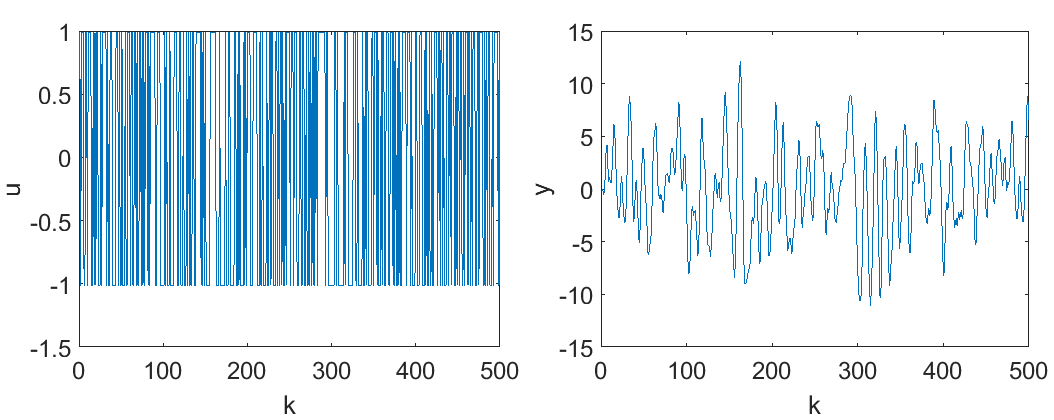
\includegraphics[scale=0.65]{18_1}

Figura $1$: Entrada e saída para modelo sem ruído.
\end{center}

\begin{center}
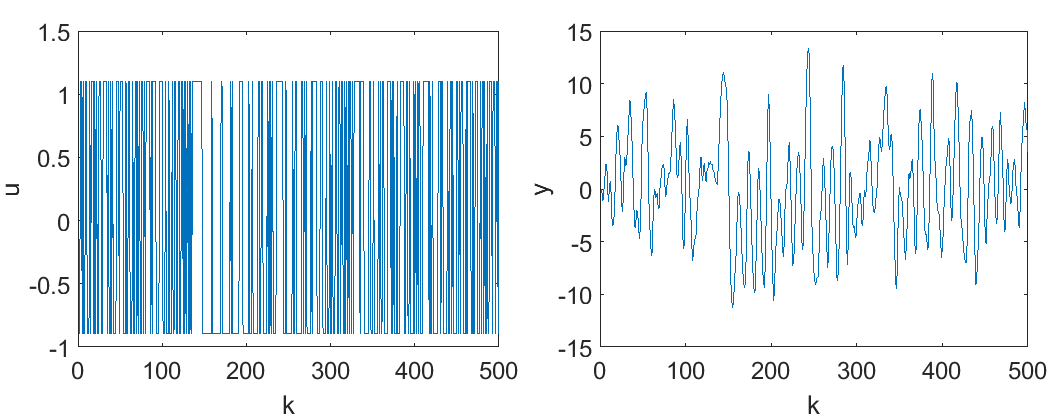
\includegraphics[scale=0.65]{18_3}

Figura $2$: Entrada e saída para modelo com ruído.
\end{center}

\begin{center}
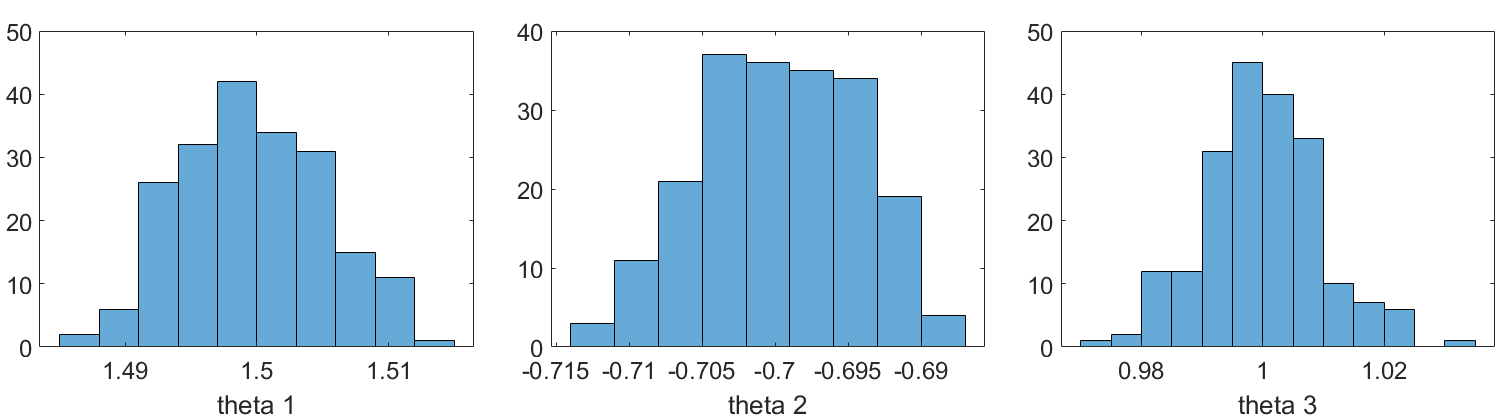
\includegraphics[scale=0.44]{18_5}

Figura $3$: Histograma baseado em $200$ execuções independentes do estimador MQ, com a mesma entrada da figura anterior.
\end{center}

\section*{Questão 2 --- versus 4.19}

Na Lista de Exercícios $2$, item $4$ os dados no arquivo prbsa02.dat
foram usados. Use agora os mesmos dados, mas para estimar um modelo
ARX. Valide seus resultados. Compare os procedimentos (em termos de
praticidade) seguidos na Lista de Exercícios $2$ e neste item.

\dotfill

Refiz a questão $4.19$, agora considerando o regime permanente: de $t = 3000$ em diante. É quase a metade final dos dados. prbsa02$(1476:2940)$.

O arquivo prbsa02.dat tem três colunas: $t,u,y$. Verificando, obtivemos a Figura $4$.

Calculamos as correlações utilizadas na equação de Wiener-Hopf e obtivemos a Figura $5$.

Plotamos a resposta ao impulso estimada versus a primeira coluna $(t)$ e obtivemos a Figura $6$.

\begin{center}
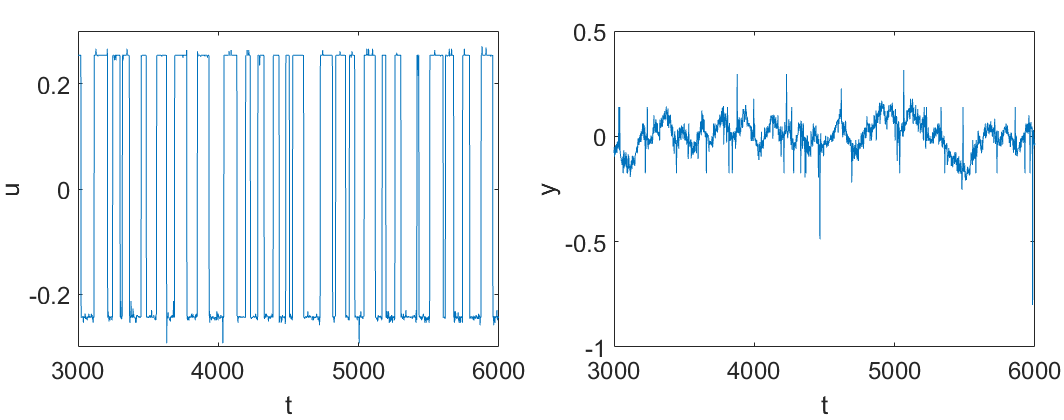
\includegraphics[scale=0.65]{4uy}

Figura $4$: Dados de prbsa02.dat
\end{center}

\newpage

\begin{center}
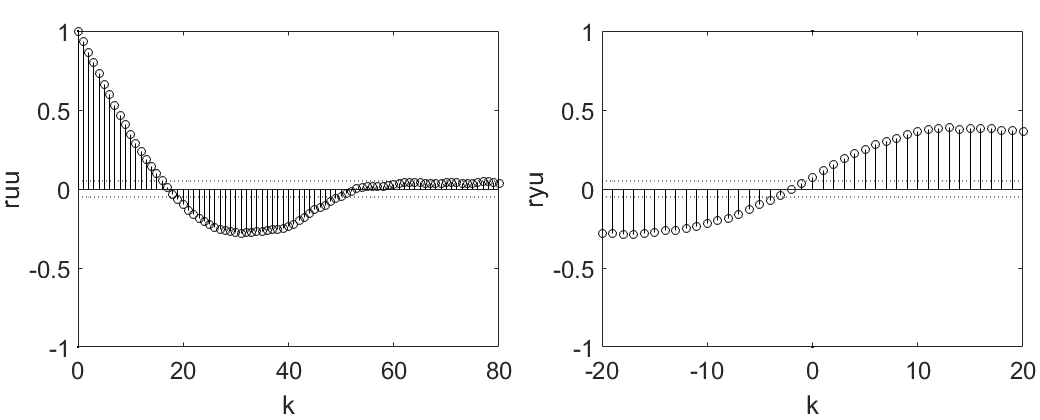
\includegraphics[scale=0.65]{4ruu}

Figura $5$: (a) Autocorrelação de $u$. (b) Correlação cruzada.
\end{center}

\begin{center}
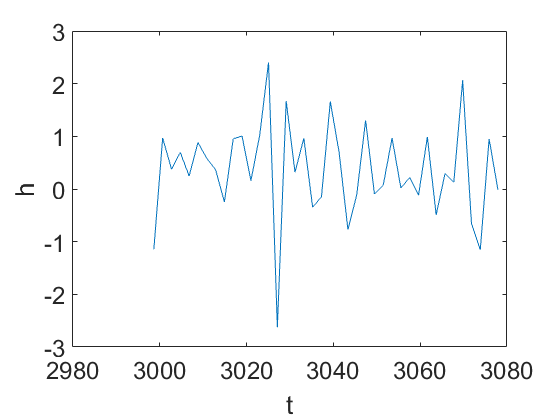
\includegraphics[scale=0.666]{4h}

Figura $6$: Resposta ao impulso estimada
\end{center}

\dotfill

Após subtrair a média, estimei $\Delta y = y_{ss} - y_0$, ou seja, a diferença entre o valor de estado estacionário e o inicial. Utilizei as aproximações: $\Delta u = 1$ e $\Delta y = y_{2940}$. Dessa forma, o valor final passa a ser $y_{ss} = 1$.

Gerei a matriz de regressores, considerando o seguinte modelo ARX:

$y(k) + a_1 y(k-1) + a_2 y(k-2) + a_3 y(k-3) = b_1 u(k - 1) + b_2 u(k - 2) + b_3 u(k - 3)$.

Para validar, fiz uma simulação com os parâmetros obtidos. A comparação entre os dados e a simulação (Figura $7$) não foi boa. Foi extraído o ruído?

A Figura $8$ mostra apenas a saída da simulação.

Para comparar com o que fiz na questão $4.19$, tornei a simular com a entrada igual a um impulso. A comparação (Figura $9$) mostrou dois sinais completamente diferentes.

\begin{center}
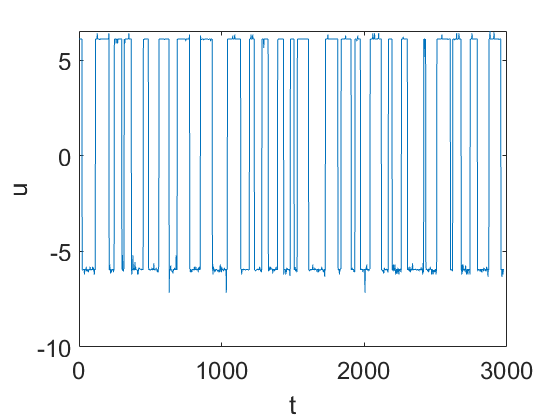
\includegraphics[scale=0.5]{2b1}
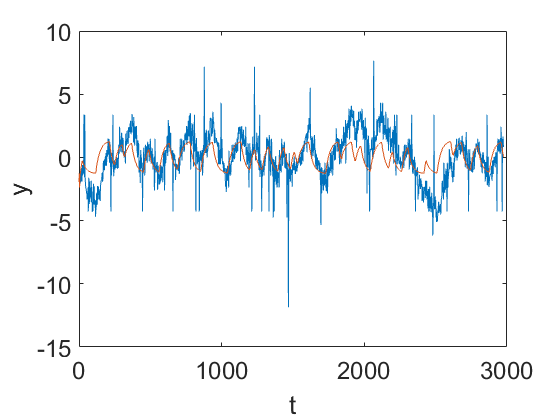
\includegraphics[scale=0.5]{2b2}

Figura $7$: (a) Entrada (b) Dados de saída em azul e saída ARX estimada em vermelho. 
\end{center}

\begin{center}
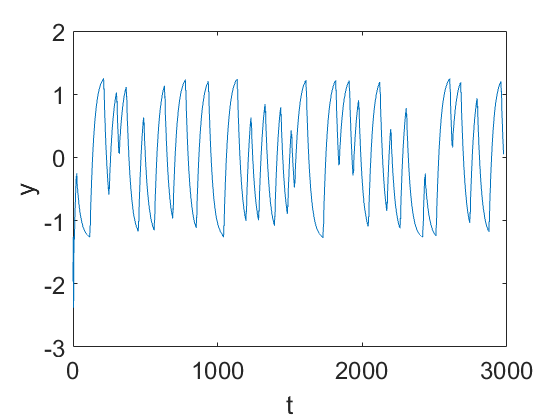
\includegraphics[scale=0.666]{2b3}

Figura $8$: Saída ARX estimada. 
\end{center}

\newpage

\begin{center}
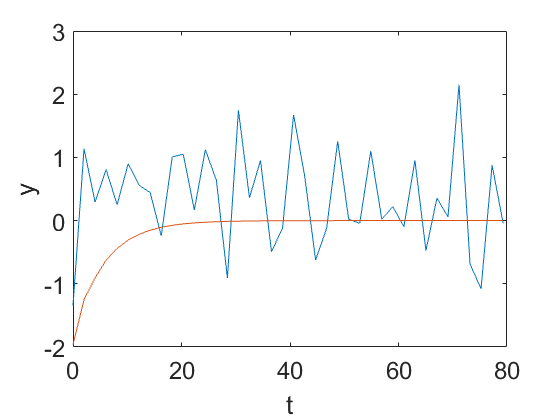
\includegraphics[scale=0.65]{2b4}

Figura $9$: Em azul a resposta ao impulso por correlações; em vermelho, a resposta ao impulso via matriz de regressores. 
\end{center}

\section*{Questão 5.13}

Os dados do arquivgo bfg33.dat são exibidos na Figura $10$.

Para retirar o offset, desconsiderei os $28$ pontos iniciais.

Estimei $\Delta y = y_{ss} - y_0$, ou seja, a diferença entre o valor de estado estacionário e o inicial.

Dividi $u$ e $y$ por $\Delta y$, a fim de que $y_{ss} = 1$. A nova entrada é exibida na Figura $11$.

Gerei a matriz de regressores, considerando o seguinte modelo ARX:

$y(k) + a_1 y(k-1) + a_2 y(k-2) = b_1 u(k - 19) + b_2 u(k - 20)$, uma vez que a primeira saída considerável para fins de atraso puro de tempo aconteceu em $k = 21$.

Fiz a simulação com os parâmetros estimados, obtive a figura $12a$. A entrada foi constante e igual a $\Delta u$. Dividi a saída por $\Delta y$.

Comparei com $H_1(s)$ e obtive a figura $12b$. Esta ficou ótima, como esperado; a anterior ficou um pouco mal aproximada em relação a $H_1$, mas bem próxima. Portanto o modelo ARX teve bom desempenho nesse caso.

\begin{center}
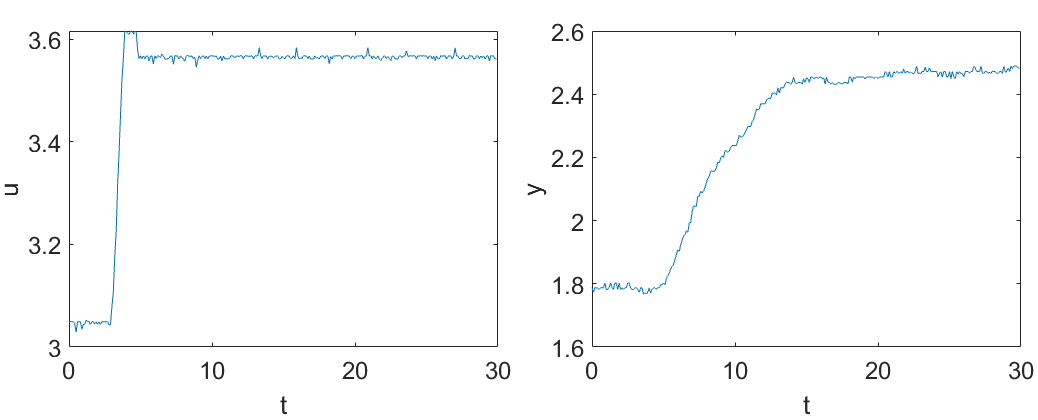
\includegraphics[scale=0.65]{33_1}

Figura $10$: Entrada e saída de bfg33.dat
\end{center}

\begin{center}
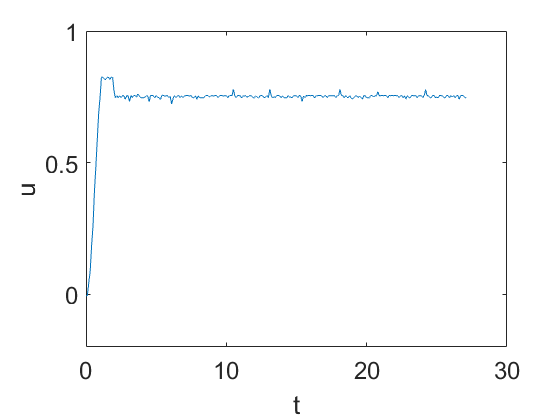
\includegraphics[scale=0.65]{33_3}

Figura $11$: Entrada considerada para os cálculos
\end{center}

\begin{center}
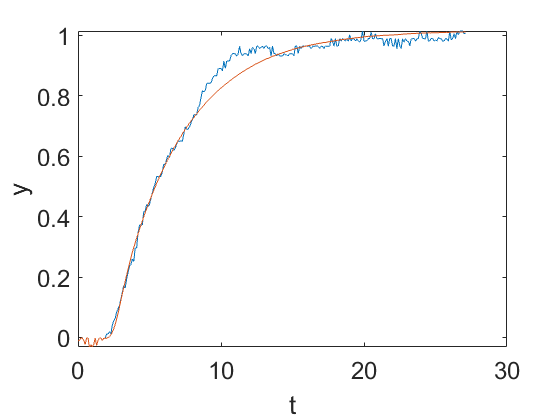
\includegraphics[scale=0.5]{33_4}
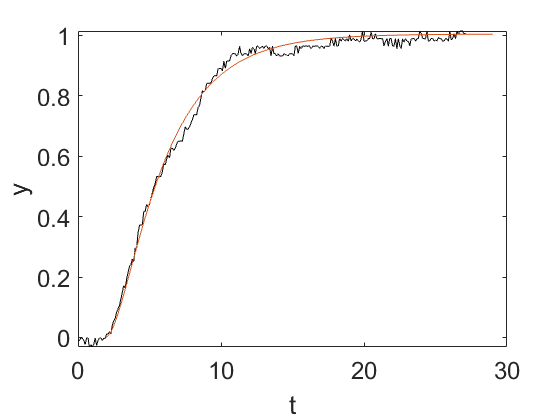
\includegraphics[scale=0.5]{33_5}

Figura $12$: a) Simulação pelo estimador MQ b) Comparação com $H_1(s)$
\end{center}

\dotfill

\newpage

Os dados do arquivgo bfg44.dat são exibidos na Figura $13$.

Para retirar o offset, não foi necessário retirar nenhum ponto inicial. Tomei o módulo de $\Delta y$.

Estimei $\Delta y = y_{ss} - y_0$, ou seja, a diferença entre o valor de estado estacionário e o inicial.

Dividi $u$ e $y$ por $\Delta y$, a fim de que $y_{ss} = 1$. A nova entrada é exibida na Figura $14$.

Gerei a matriz de regressores, considerando o seguinte modelo ARX:

$y(k) + a_1 y(k-1) + a_2 y(k-2) = b_1 u(k - 32) + b_2 u(k - 33)$, uma vez que a primeira saída considerável aconteceu em $k = 34$, quando é decrescente.

Fiz a simulação com os parâmetros estimados, obtive a figura $15a$. A entrada foi constante e igual a $\Delta u$. Dividi a saída por $\Delta y$.

Comparei com $H_2(s)$ e obtive a figura $15b$. Esta ficou como esperado pelo exemplo; a anterior ficou péssima em relação a $H_2$. Portanto o modelo ARX teve desempenho ruim nesse caso. A fim de melhorar, poderíamos aumentar a quantidade de colunas da matriz regressora; melhor ainda, considerar este sistema como não linear e utilizar métodos mais sofisticados.

A forma dos sinais $H_i$ é $H_i(s) = \cfrac{K e^{-\tau_d s}}{(\tau_1 s + 1)(\tau_2 s + 1)}$. Nós comparamos com modelos ARX cuja transformada $Z$ é $Y(z) + a_1 \cfrac{Y(z)}{z} + a_2 \cfrac{Y(z)}{z^2} = b_1 \cfrac{U(z)}{z^{n-1}} + b_2 \cfrac{U(z)}{z^n}$. A maior dificuldade é encontrar o grau de $A(q)$ e $B(q)$, e a quantidade de regressores de ambos, que minimiza a função objetivo. Com mais esforço e tempo, conseguiríamos estimar exatamente os parâmetros $H_1(z)$ e $H_2(z)$, devidamente discretizados ou amostrados.

\begin{center}
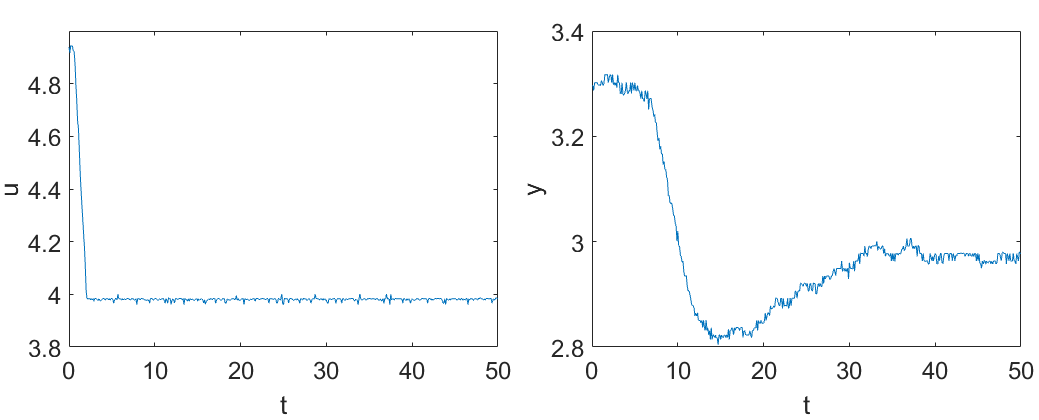
\includegraphics[scale=0.65]{44_1}

Figura $13$: Entrada e saída de bfg44.dat
\end{center}

\begin{center}
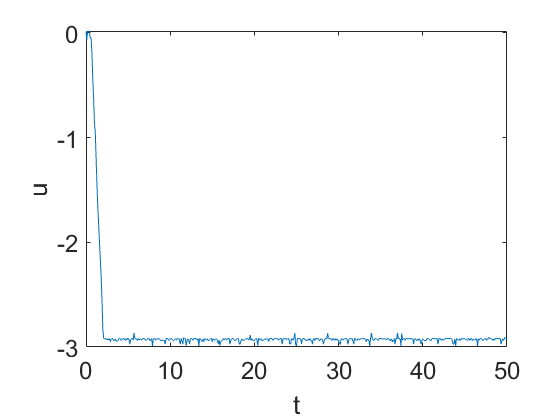
\includegraphics[scale=0.65]{44_3}

Figura $14$: Entrada considerada para os cálculos
\end{center}

\begin{center}
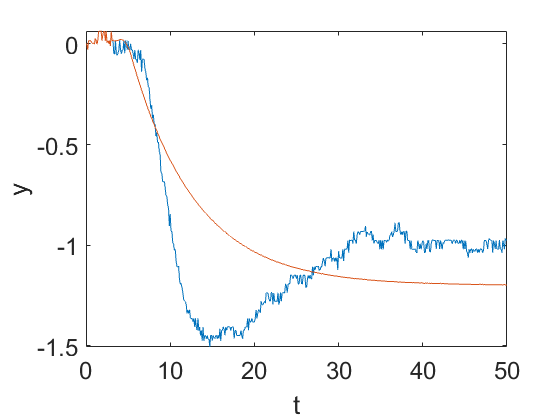
\includegraphics[scale=0.5]{44_4}
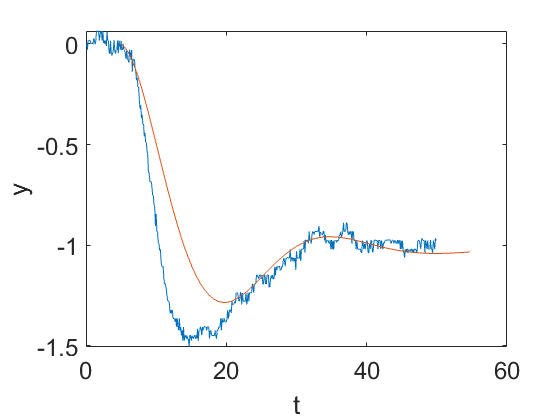
\includegraphics[scale=0.5]{44_5}

Figura $15$: a) Simulação pelo estimador MQ b) Comparação com $H_2(s)$
\end{center}

\newpage

Para terminar, gerei nova matriz de regressores, considerando o seguinte modelo ARX:

$y(k) + \sum_{i=1}^5 a_i y(k-i) = \sum_{j = 29}^{33} b_j u(k - j)$. O resultado está exibido na Figura $16$ e foi bem aproximado apenas no início, indicando possível mudança de ponto de operação.

\begin{center}
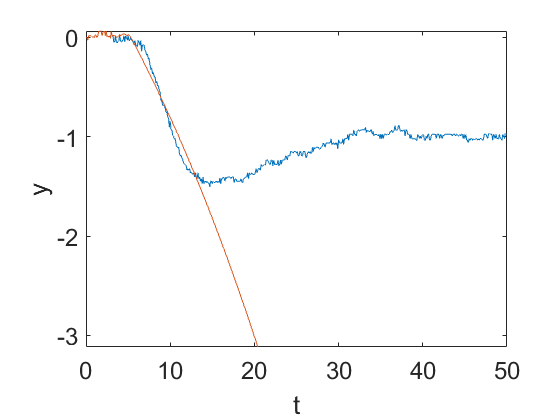
\includegraphics[scale=0.666]{44b}

Figura $16$: Nova simulação com matriz de dez colunas
\end{center}

\vspace{6mm}

Link para os \href{https://drive.google.com/file/d/1c9wNTYZ-MPxCvBaisc35zPRq-oZGPTos/view?usp=sharing}{\color{blue}\underline{códigos-fonte}}.

Versão de 20/maio/2022\footnote{Fora da caridade não há salvação.} por Vinicius Claudino Ferraz. 

Matrícula: 2019435823.

\end{document}
